\section{Quest Package}
%TODO referenz folgt Quest Package erklärung
Hier kann man zwischen den vorhanden Quest Packages wählen. Wobei rechts die Beschreibung des jeweiligen Packages, falls diese vorhanden ist, angezeigt wird. Mithilfe eines Klicks auf den Pfeil kann das gewünschte Package ausgewählt werden.

Weiters wird auch der Fortschritt des Packages angezeigt. Daraus ist ersichtlich, wie viele Quests man in diesem Packet bereits fertiggestellt wurden.

Bei einem Quest Package wurde ein JTree\footnote{\url{http://www.hameister.org/JavaSwingTreeTable.html}}  zur Realisierung verwendet. Dieses befindet sich wiederum in einer JScrollpane. Somit ist die Anzahl der Elemente in der JTable\footnote{\url{https://docs.oracle.com/javase/tutorial/uiswing/components/scrollpane.html}}  , und somit eines Packages, nicht begrenzt.

\subsection{Auslesen der Packages}
\begin{figure}[h] 
  \centering
     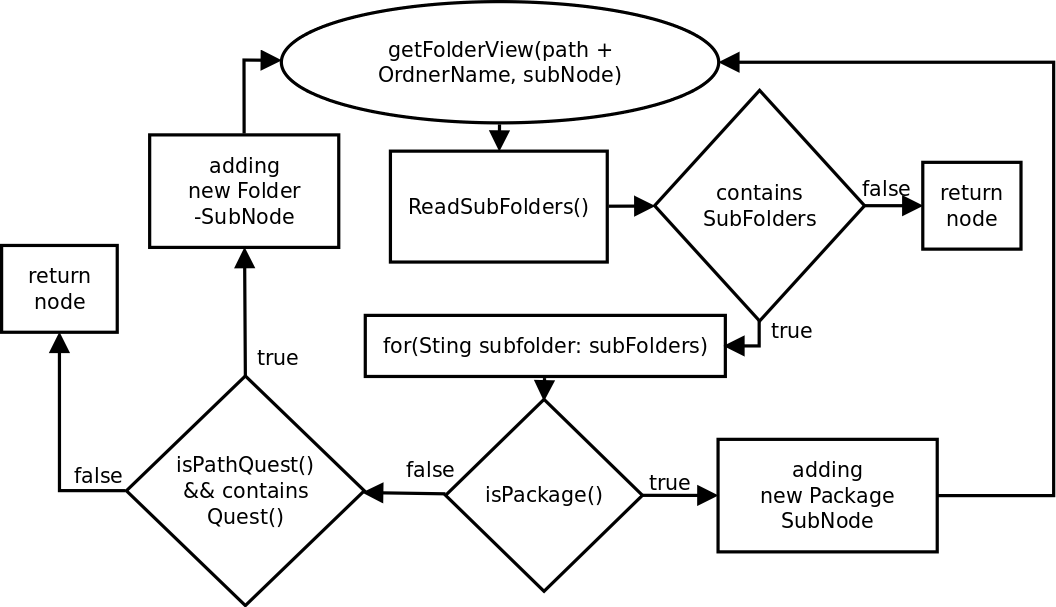
\includegraphics[width=1\textwidth]{./media/images/gui/package-tree-rekursion.png}
  \caption{Schematische Darstellung vom Auslesen der Packages}
  \label{fig:Package_Tree_Rekursion}
\end{figure}


Ob ein Ordner ein Package ist, wird mithilfe einer Rekursion ausgelesen. Der Ausgangspunkt dieser Rekursion bildet der Ordner \textbf{"`packages"'}. Dieser bildet auch den Haupt-Knoten. Nun wird \textit{\textbf{getFolderView()}} aufgerufen, und der relative Pfad und der Hauptknoten werden übergeben.

Von diesem Punkt aus wird in die nächsten Unterordner gewechselt. Dort wird nun zuerst überprüft, ob der gewählte Ordner Subordner enthält. Ist dies der Fall, wird durch die Liste der Unterordner mithilfe einer ForEach-Schleife durchiteriert.

Es wird nun überprüft, ob eines dieser Elemente ein Package ist. Trifft dies zu, wird das gerade iterierende Element als Unterknoten hinzugefügt und dieselbe Methode (\textit{\textbf{getFolderView()}}) wird nochmals aufgerufen.

Wenn das aktuelle Element kein Package ist, erfolgt erneut eine Überprüfung nach weiteren Quests im Unterordner. Werden solche gefunden, wird ein neuer Unterknoten erstellt und wiederum die eigene Methode aufgerufen.

Wenn diese Bedingung nicht zutrifft, wird der Hauptknoten wieder zurückgegeben.

\subsection{Überprüfungs - Iterationen und Rekursion}
Da eine Quest eine \textit{ref.cmm}, \textit{description.html} und eine \textit{input.cmm} haben muss, ist es möglich, anhand einer Iteration festzustellen, ob es sich bei diesen Ordnern um Quests handelt.

Durch eine einfache Rekursion kann der gesamte Ordner mit seinen Unterordnern aufgeschlüsselt beziehungsweise auf Quests überprüft werden.

\textit{\textbf{isPathQuest(path)}}, überprüft hierbei, ob der Ordner eine Quest ist.
\begin{lstlisting}[language=JAVA]
	public static boolean containsQuests(String path){
		//Checking if there is a Quest in the Current Folder
		if(isPathQuest(path))
			return true;
		//Iterate Through all other Folders
		else{
			List<String> subFolders = Quest.ReadFolderNames(path);
			if(subFolders != null){
				for(String subFolder : subFolders){
						return containsQuests(path + File.separator + subFolder);
				}
			}
		}
		return false;
	}
\end{lstlisting}



\begin{figure}[h] 
  \centering
     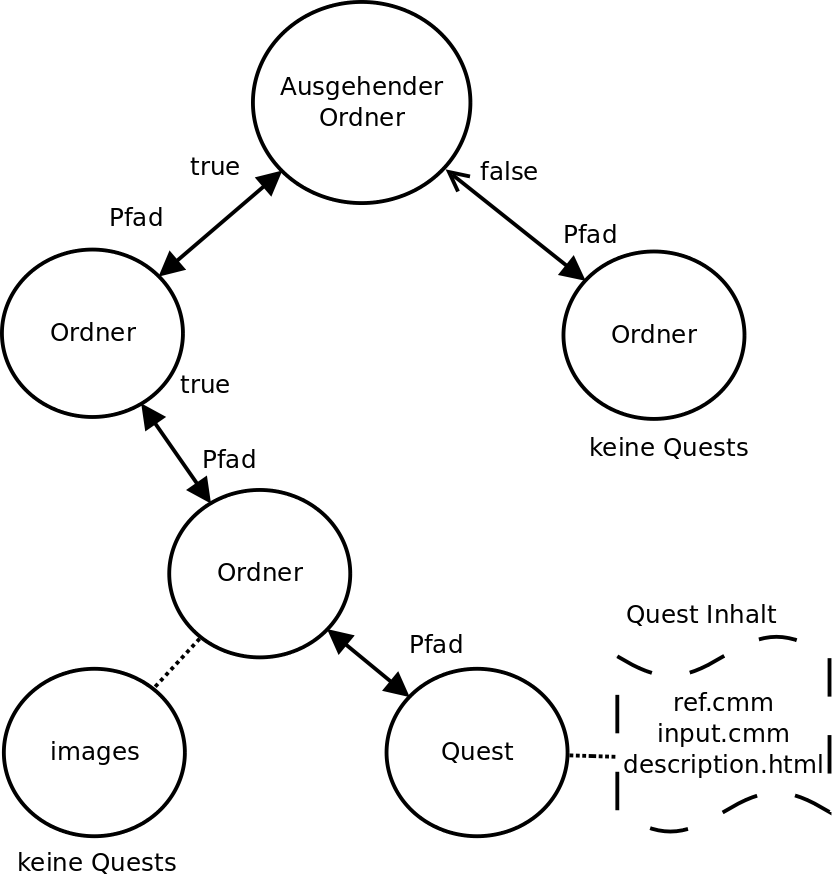
\includegraphics[width=0.5\textwidth]{./media/images/gui/quest-control-rekursion.png}
  \caption{Schematische Darstellung der Rekursion}
  \label{fig:JTree_Control_Rekursion}
\end{figure}

In der Abbildung \ref{fig:JTree_Control_Rekursion} wird ein beispielhafter Ordnerpfad aufgeschlüsselt. Der Ordner oberhalb des Questordners kann nun als Package erkannt werden.